%% ---------------------------------------------------------------------
%% 03 - DỮ LIỆU THỰC NGHIỆM VÀ PHÂN TÍCH KHÁM PHÁ
%% ---------------------------------------------------------------------

\section{Dữ liệu thực nghiệm và phân tích khám phá}\label{sec:data}

Bài toán của nghiên cứu là bài toán hình học -- tối ưu trong không gian ba chiều,
không thuộc lớp bài toán học máy có giám sát: ``dữ liệu'' ở đây là các \textbf{bề
mặt đa diện tam giác hóa} (mesh) mà đường đi ngắn nhất trắc địa được tính toán
trên đó, kèm theo các tập \textbf{kết quả tham chiếu} dùng để đối chiếu và kiểm
chứng tính đúng đắn của thuật toán.

Toàn bộ dữ liệu thực nghiệm, mã nguồn thuật toán và công cụ hỗ trợ được công khai
tại \cite{kien2026repo}. Dữ liệu được tổ chức thành ba lớp: \emph{nguồn gốc} gồm
9 mesh \texttt{.off} và scene thành phố \texttt{city.glb}; \emph{đã xử lý} gồm
mesh đã kiểm tra, bề mặt dẫn đường và mission START/GOAL; và \emph{tham chiếu} gồm
5 tệp polyline cho các mesh nhỏ. Kết quả của mỗi lần chạy được lưu riêng, không
ghi đè lên lần trước. Đường dẫn tệp cụ thể nằm ở Phụ lục A.

Mục này mô tả chi tiết hai nguồn dữ liệu thực nghiệm, định dạng và data dictionary
của chúng, kết quả kiểm tra chất lượng dữ liệu, phân tích khám phá (EDA) kèm trực
quan hóa hình ảnh không gian 3D, từ đó rút ra các insight ảnh hưởng trực tiếp tới
khâu đánh giá thực nghiệm ở Mục~\ref{sec:results}.

\subsection{Nguồn dữ liệu}

\begin{enumerate}
\item Bộ mesh kiểm thử gồm 9 tệp \texttt{.off} dạng văn bản thuần:
\begin{itemize}
  \item 5 mesh mẫu có đường tham chiếu độc lập dùng để đối chiếu kết quả: \texttt{J17}, \texttt{L}, \texttt{cliff},
    \texttt{demo\_mesh}, \texttt{star}. Đây là các mesh tổng hợp nhỏ (khối đa diện
    lồi, ``đồi vách dốc'', lưới mẫu không lồi).
  \item 2 mesh dựng lại theo hình minh họa của bài báo gốc \cite{an2024funnel}:
    \texttt{cube} (Hình~7 của bài báo) và \texttt{icosahedron} (Hình~4 của bài
    báo).
  \item 2 mesh mở rộng cho bề mặt mở: \texttt{dome} (mảnh vỏ cầu hở khuyết đáy có
    8 cạnh biên) và \texttt{terrain} (mô hình địa hình có thung lũng lõm và 24
    cạnh biên).
  \item kèm theo là file mô hình thành phố \texttt{city.glb} (khoảng 20,5 MB, mô
    hình 3D định dạng glTF/GLB), được dùng cho quy trình mô phỏng ở
    Mục~\ref{sec:gazebo}.
\end{itemize}

\item Kết quả tham chiếu gồm 5 tệp JSON cho các mesh \texttt{cliff},
  \texttt{demo\_mesh}, \texttt{J17}, \texttt{L} và \texttt{star}; mỗi tệp ghi
  \texttt{mesh}, \texttt{source},
  \texttt{coordinate\_system} và danh sách \texttt{paths}; \texttt{paths[i]} là
  polyline ngắn nhất từ đỉnh nguồn tới đỉnh $i$, tọa độ các điểm uốn trắc địa làm
  tròn 4 chữ số thập phân. Hai mesh \texttt{cube} và \texttt{icosahedron} được
  dựng theo hình vẽ của bài báo gốc, còn \texttt{dome} và \texttt{terrain} là hai
  bề mặt mở; bốn mesh này không có file tham chiếu độc lập trong repo, nên được
  dùng để kiểm tra khả năng chạy và tính nhất quán nội tại chứ không đối chiếu
  từng đỉnh.
\end{enumerate}

Bộ mesh kiểm thử có tính đại diện vì gồm các mesh tổng hợp với kích thước từ 7 đến
49 đỉnh. Mặc dù nhỏ hơn quy mô 100--800 đỉnh trong bài báo \cite{an2024funnel},
tập dữ liệu này bao quát đầy đủ các dạng cấu trúc hình học đặc trưng: đa diện lồi,
bề mặt không lồi, bề mặt có lỗ (xuyến $\chi=0$) và bề mặt mở có cạnh biên
($\chi=1$). Nhờ đó, tập dữ liệu đáp ứng yêu cầu kiểm chứng tính đúng đắn và độ ổn
định của thuật toán.

\subsection{Mô tả dữ liệu và Data Dictionary}

File đầu vào có định dạng \texttt{.off} và được đọc bởi một hàm đọc mesh duy nhất.
Dòng đầu là \texttt{OFF}; dòng thứ hai gồm ba số
nguyên \texttt{V F E} ($V$ = số đỉnh, $F$ = số mặt tam giác, $E$ = số cạnh); tiếp
theo là $V$ dòng tọa độ thực \texttt{x y z}; cuối cùng là $F$ dòng tam giác
\texttt{3 i j k} (ba chỉ số đỉnh, đánh chỉ mục từ 0). Trường $E$ trong một số file
không chính xác và được tính lại từ danh sách tam giác. Kết quả tham chiếu có định
dạng JSON, trong đó mỗi phần tử của danh sách \texttt{paths} là một polyline 3D ứng với một đỉnh đích; tọa độ được làm tròn 4
chữ số thập phân.

Vì dữ liệu là mesh đa diện 3D chứ không phải bảng dữ liệu quan sát dạng dòng/cột
truyền thống, các ``biến'' ở đây là các \textbf{đặc trưng cấu trúc hình học và tô
pô của mesh}. Bảng~\ref{tab:data-dictionary} định nghĩa chi tiết Data Dictionary.

\begin{table*}[!t]
  \caption{Data Dictionary của bộ mesh kiểm thử.}
  \label{tab:data-dictionary}
  {\fontsize{7}{8.6}\selectfont
  \setlength{\tabcolsep}{3pt}%
  \begin{adjustbox}{max width=\textwidth}
  \begin{tabular}{@{}>{\raggedright\arraybackslash}p{54pt}
                  >{\raggedright\arraybackslash}p{52pt}
                  >{\raggedright\arraybackslash}p{146pt}
                  >{\raggedright\arraybackslash}p{36pt}
                  >{\raggedright\arraybackslash}p{104pt}@{}}
    \toprule
    \textbf{Biến} & \textbf{Kiểu dữ liệu} & \textbf{Ý nghĩa} & \textbf{Đơn vị} &
    \textbf{Vai trò} \\
    \midrule
    \texttt{name} & chuỗi & tên file mesh (\texttt{cliff.off}, \ldots) & --- &
      định danh \\
    $V$ & nguyên & số đỉnh của mesh & đỉnh & quy mô; chi phối độ phức tạp
      $O(V^2)$ \\
    $F$ & nguyên & số mặt tam giác & tam giác & quy mô \\
    $E$ & nguyên & số cạnh khác nhau (tính từ danh sách tam giác) & cạnh & kiểm tra
      nhất quán Euler \\
    $\chi=V-E+F$ & nguyên & số Euler & --- & phân loại bề mặt (kín, mở, xuyến) \\
    \texttt{boundary} & nguyên & số cạnh chỉ kề đúng 1 tam giác & cạnh & phát hiện
      bề mặt mở \\
    \texttt{components} & nguyên & số thành phần liên thông & --- & kiểm mesh rời
      rạc \\
    \texttt{span} & thực & độ rộng theo từng trục ($\max-\min$ tọa độ) & đơn vị
      mesh & phát hiện khác thang đo \\
    $s$ & nguyên & chỉ số đỉnh nguồn (0-based) & --- & điều kiện đầu vào của mỗi
      thí nghiệm \\
    \texttt{has\_expected} & logic & có đường tham chiếu độc lập hay không &
      --- & xác định phạm vi kiểm chứng \\
    \bottomrule
  \end{tabular}
  \end{adjustbox}}
\end{table*}

Bảng~\ref{tab:dac-trung-mesh} áp dụng Data Dictionary này cho toàn bộ 9 mesh kiểm
thử \cite{kien2026repo}.

\begin{table*}[!t]
  \caption{Đặc trưng hình học và tô pô của 9 mesh kiểm thử.}
  \label{tab:dac-trung-mesh}
  {\fontsize{7}{8.6}\selectfont
  \setlength{\tabcolsep}{2.5pt}%
  \begin{adjustbox}{max width=\textwidth}
  \begin{tabular}{@{}lrrrrrlr@{}}
    \toprule
    \textbf{Mesh} & $V$ & $F$ & $E$ & $\chi$ & \textbf{Cạnh biên} &
    \textbf{Dạng bề mặt} & \textbf{Tham chiếu} \\
    \midrule
    \texttt{cliff}        & 7  & 10 & 15  & 2 & 0  & Kín (cầu)       & \texttt{paths.json} \\
    \texttt{cube}         & 8  & 12 & 18  & 2 & 0  & Kín (lồi)       & Không có \\
    \texttt{J17}          & 10 & 16 & 24  & 2 & 0  & Kín (cầu)       & \texttt{paths.json} \\
    \texttt{L}            & 12 & 20 & 30  & 2 & 0  & Kín (cầu)       & \texttt{paths.json} \\
    \texttt{icosahedron}  & 12 & 20 & 30  & 2 & 0  & Kín (lồi đều)   & Không có \\
    \texttt{star}         & 16 & 28 & 42  & 2 & 0  & Kín (không lồi) & \texttt{paths.json} \\
    \texttt{dome}         & 25 & 40 & 64  & 1 & 8  & Mở (vỏ cầu)     & Không có \\
    \texttt{demo\_mesh}   & 31 & 62 & 93  & 0 & 0  & Kín (xuyến)     & \texttt{paths.json} \\
    \texttt{terrain}      & 49 & 72 & 120 & 1 & 24 & Mở (địa hình)   & Không có \\
    \bottomrule
  \end{tabular}
  \end{adjustbox}
  \vspace{2pt}

  \footnotesize\raggedright
  Cột $\chi=V-E+F$ là số Euler. ``Không có'' nghĩa là mesh không có file tham
  chiếu độc lập; các mesh này được dùng để kiểm tra
  khả năng chạy trên bề mặt lồi, bề mặt mở và bề mặt có lỗ, không đối chiếu từng
  đỉnh.}
\end{table*}

\subsection{Đánh giá chất lượng dữ liệu}

Các kiểm tra tự động trên cả 9 file đầu vào (thực hiện bởi bộ đọc mesh và bộ lập
tuyến):
\begin{description}
  \item[Cấu trúc hợp lệ] Mọi dòng tam giác đều có dạng \texttt{3 i j k} với
    $0\le i,j,k<V$; không có chỉ số đỉnh nào nằm ngoài phạm vi, không có tam giác
    nào bị thiếu đỉnh.
  \item[Trùng lặp và nhiễu] Không có đỉnh trùng tọa độ trên cả 9 mesh; không có tam
    giác thoái hóa --- diện tích tam giác nhỏ nhất trong toàn bộ dữ liệu là 0,0920
    (đơn vị vuông, trên \texttt{dome}), lớn hơn nhiều ngưỡng zero số học $10^{-12}$.
  \item[Tính hình học 2-manifold] Không có cạnh nào kề quá 2 tam giác (mesh phi đa
    tạp bằng 0); mỗi mesh tạo thành một thành phần liên thông hoàn chỉnh duy nhất.
  \item[Phân loại bề mặt kín và mở] Có 7 mesh là bề mặt kín hoàn toàn với 0 cạnh
    biên (trong đó 6 mesh có $\chi=2$ dạng cầu và \texttt{demo\_mesh} có $\chi=0$
    dạng xuyến có lỗ rỗng xuyên tâm). Hai mesh còn lại là bề mặt mở: \texttt{dome}
    có 8 cạnh biên và \texttt{terrain} có 24 cạnh biên, cả hai đều đạt số đặc
    trưng Euler $\chi=1$ đúng với cấu trúc bề mặt mở có một chu vi biên liên tục.
  \item[Nhất quán số Euler] Với mọi mesh, giá trị $V-E+F$ tính từ dữ liệu khớp
    chính xác tuyệt đối với $\chi$ ở Bảng~\ref{tab:dac-trung-mesh} (2, 1 hoặc 0),
    không xảy ra sai lệch tô pô ở bất kỳ mô hình nào.
  \item[Lỗi vô hại ở header file] Số thứ ba của dòng đầu (cột $E$ theo quy ước gốc)
    không phải lúc nào cũng chính xác trong file văn bản: ví dụ \texttt{L.off} ghi
    10 (thực tế $E=30$), \texttt{demo\_mesh.off} ghi 0 (thực tế 93). Mã nguồn đọc
    file tự động suy ra danh sách cạnh thực tế từ các mặt tam giác nên sai lệch ở
    header hoàn toàn vô hại đối với thuật toán.
  \item[Khác biệt thang đo tọa độ] 8 mesh có tọa độ trong khoảng đơn vị nhỏ, cỡ
    $[-3,5]$; riêng \texttt{demo\_mesh} trải trên $x\in[26,344]$, $y\in[-320,550]$,
    $z\in[-288,207]$ --- độ rộng lớn gấp khoảng 100 lần. Do đó, sai số tuyệt đối
    giữa các mesh không thể so sánh gộp chung mà phải dùng sai số tương đối.
\end{description}

Về tập kết quả tham chiếu, 5/9 mesh có file \texttt{.paths.json} trong
tham chiếu; bốn mesh còn lại (\texttt{cube}, \texttt{icosahedron},
\texttt{dome}, \texttt{terrain}) không có tham chiếu độc lập. Công cụ
bước đối chiếu chạy Funnel Tree từ đúng đỉnh nguồn ghi trong
reference, so độ dài từng polyline với dung sai tương đối $10^{-4}$ và hiện báo
0 failure trên tổng 76 đỉnh; sai số tương đối lớn nhất là $1{,}7\times10^{-5}$
(\texttt{cliff}), phát sinh từ việc reference chỉ giữ bốn chữ số thập phân. Với
bốn mesh không có reference, kết quả chỉ được kiểm tra nhất quán nội tại: độ dài
polyline dựng lại phải khớp độ dài nội tại mà phép lan truyền tính được, chứ
không có đối chiếu với một bộ giải thứ hai.

\subsection{Exploratory Data Analysis và trực quan hóa}

Trước khi thực hiện các phép đo chi tiết, quy trình EDA đặt ra bốn câu hỏi then
chốt đối với tập dữ liệu:
\begin{enumerate}
  \item Bộ mesh bao gồm những dạng hình học và đặc trưng tô pô nào (kín/mở,
    lồi/không lồi, có lỗ rỗng)?
  \item Quy mô đỉnh và mặt của từng mesh ra sao, có đủ đa dạng để đánh giá thuật
    toán không?
  \item Các mesh có cùng thang đo tọa độ không gian không?
  \item Nguồn kiểm chứng chuẩn phủ bao nhiêu phần của bộ mesh?
\end{enumerate}
Tổng hợp từ Bảng~\ref{tab:dac-trung-mesh} và phần phân tích chất lượng dữ liệu:
\begin{description}
  \item[Đặc trưng tô pô (Q1)] Đa dạng cao: 7 mesh kín (6 dạng cầu $\chi=2$, 1 dạng
    xuyến $\chi=0$) và 2 mesh mở có cạnh biên ($\chi=1$).
  \item[Quy mô mesh (Q2)] Số đỉnh $V$ trải từ 7 đến 49 (trung vị 12), số mặt $F$
    từ 10 đến 72 (trung vị 20), số cạnh $E$ từ 15 đến 120. Tập mesh có độ dãn quy
    mô hợp lý để kiểm chứng thuật toán từ đơn giản đến phức tạp.
  \item[Thang đo không gian (Q3)] 8 mesh dùng bậc đơn vị cỡ 1--5; riêng
    \texttt{demo\_mesh} dùng bậc $10^2$ (lệch khoảng 100 lần).
  \item[Phủ chuẩn kiểm chứng (Q4)] 5 mesh có file tham chiếu
    đường tham chiếu; 4 mesh còn lại (\texttt{cube},
    \texttt{icosahedron}, \texttt{dome}, \texttt{terrain}) chỉ kiểm tra được
    khả năng chạy và tính nhất quán nội tại.
\end{description}

Các hình dưới đây được kết xuất trực tiếp từ công cụ trực quan hóa của quy
trình; mỗi ảnh có chân ghi tham số, số đỉnh/mặt và SHA của mesh.
Hình~\ref{fig:closed-meshes} trực quan hóa ba mô hình lưới đa diện kín tiêu biểu:
khối đa diện lồi đều \texttt{icosahedron}, mô hình vách dốc \texttt{cliff} và khối
sao không lồi \texttt{star}.

\begin{figure*}[!t]
  \centering
  \begin{subfigure}{0.46\textwidth}
    \centering
    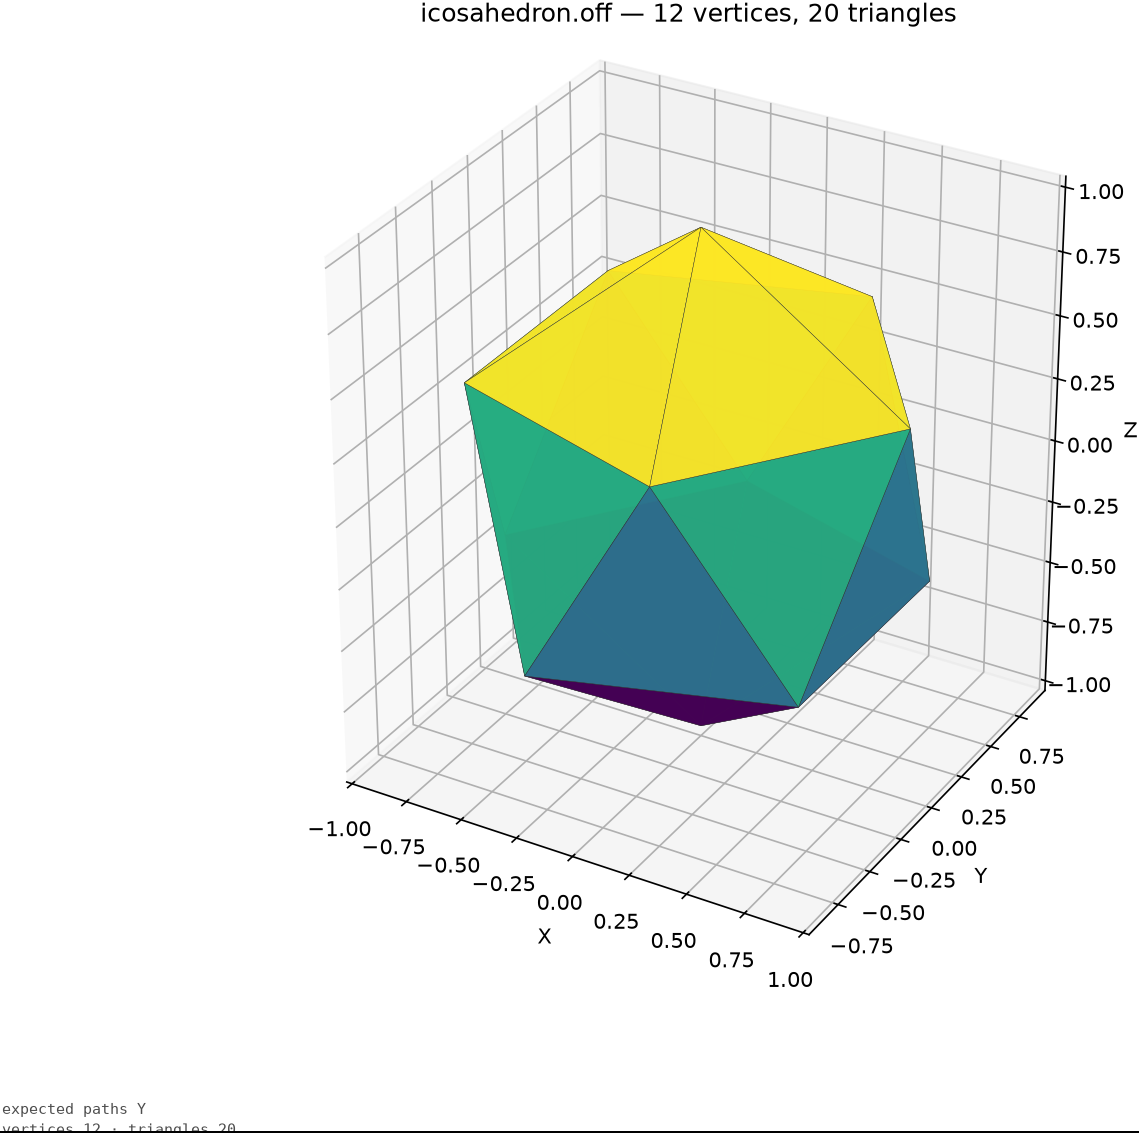
\includegraphics[width=\linewidth]{Figures/crop/repo_icosahedron.png}
    \caption{\texttt{icosahedron} ($V=12$, $F=20$)}
  \end{subfigure}\hfill
  \begin{subfigure}{0.46\textwidth}
    \centering
    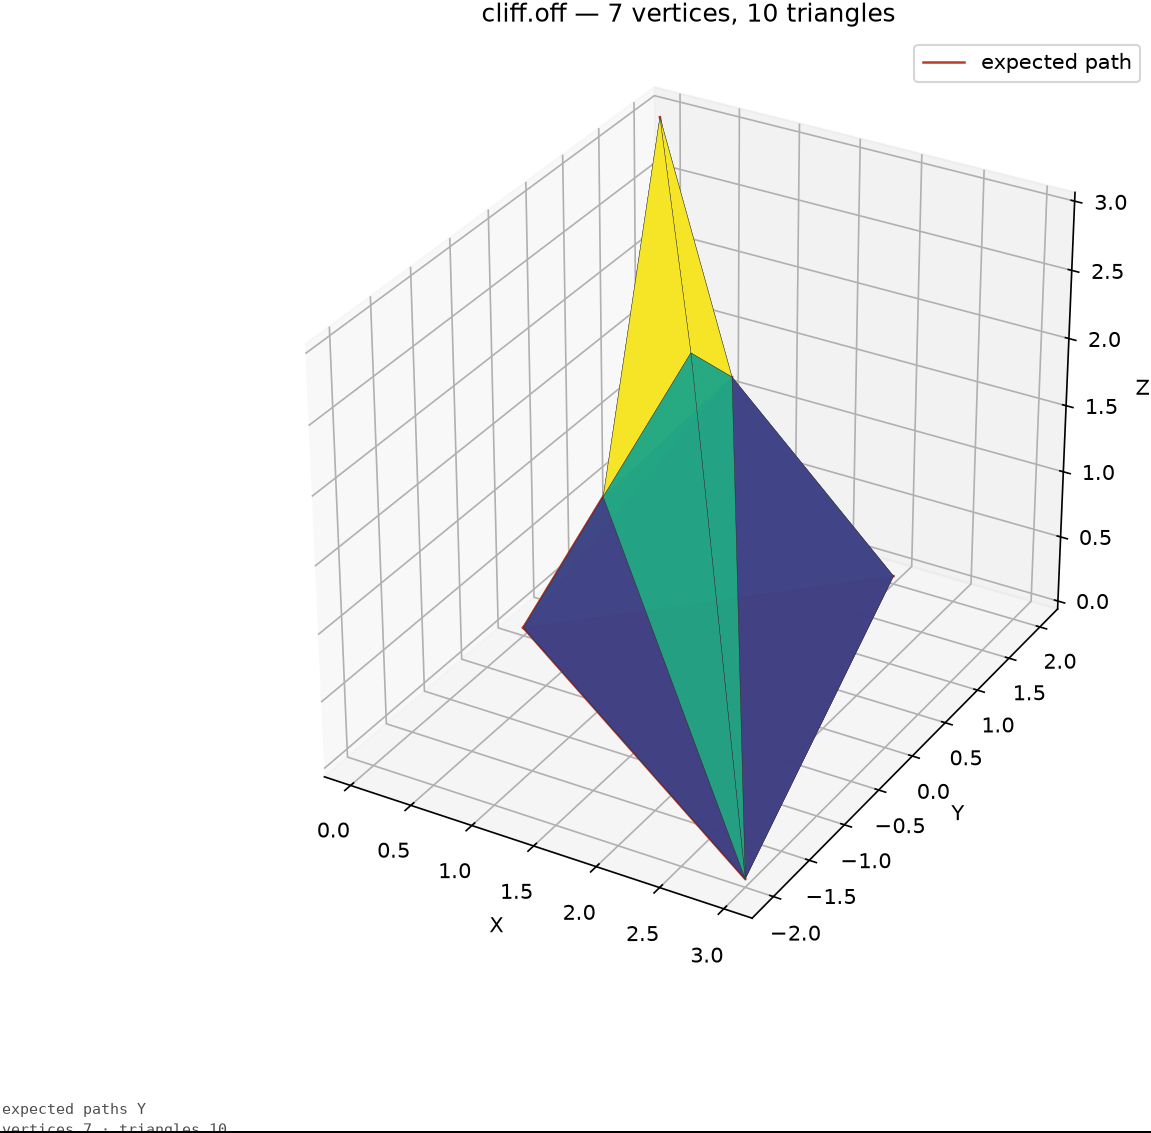
\includegraphics[width=\linewidth]{Figures/crop/repo_cliff.png}
    \caption{\texttt{cliff} ($V=7$, $F=10$)}
  \end{subfigure}\par\vspace{2pt}
  \begin{subfigure}{0.46\textwidth}
    \centering
    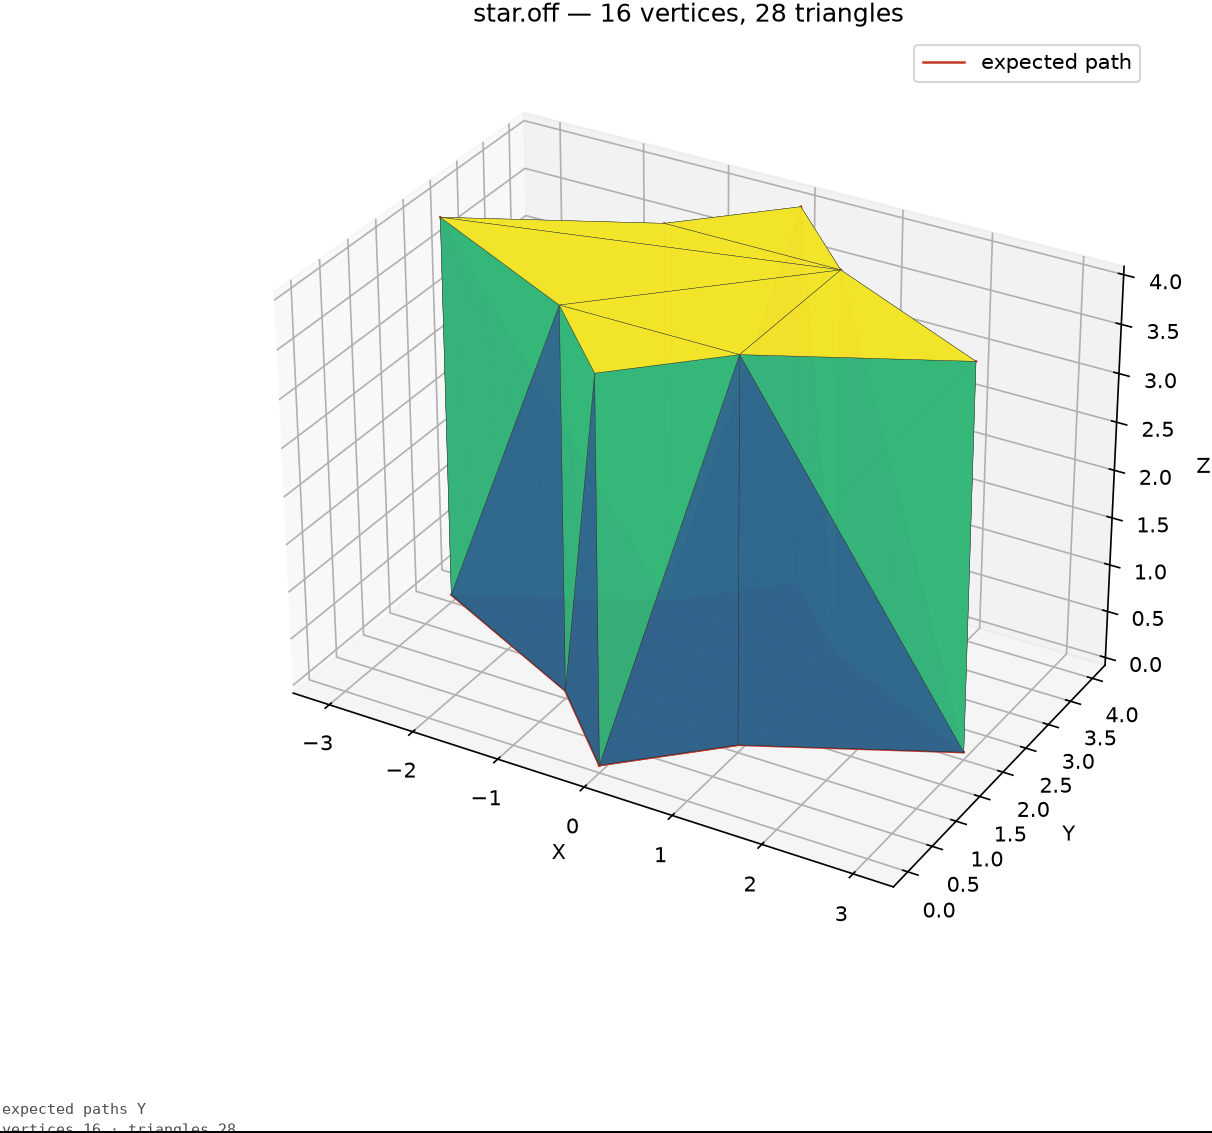
\includegraphics[width=\linewidth]{Figures/crop/repo_star.png}
    \caption{\texttt{star} ($V=16$, $F=28$)}
  \end{subfigure}
  \caption{Trực quan hóa một số lưới đa diện bề mặt kín tiêu biểu, kết xuất từ
    công cụ trực quan hóa.}
  \label{fig:closed-meshes}
\end{figure*}

Hình~\ref{fig:closed-meshes} cho thấy ba dạng hình học rất khác nhau: khối
icosahedron lồi đều với các mặt tam giác, \texttt{cliff} có một vách dốc và các
sườn nghiêng, còn \texttt{star} lõm với các múi nhọn. Sự khác biệt này là cơ sở
để kiểm tra thuật toán trên cả bề mặt lồi và không lồi.

Hình~\ref{fig:closed-meshes-2} tiếp tục trực quan hóa ba mô hình bề mặt kín còn
lại của bộ dữ liệu: khối lập phương \texttt{cube}, và hai mesh có dữ liệu đối
chiếu chuẩn là \texttt{J17} và \texttt{L}. Như vậy,
cả bảy mesh bề mặt kín đều được thể hiện trực quan đầy đủ.

\begin{figure*}[!t]
  \centering
  \begin{subfigure}{0.46\textwidth}
    \centering
    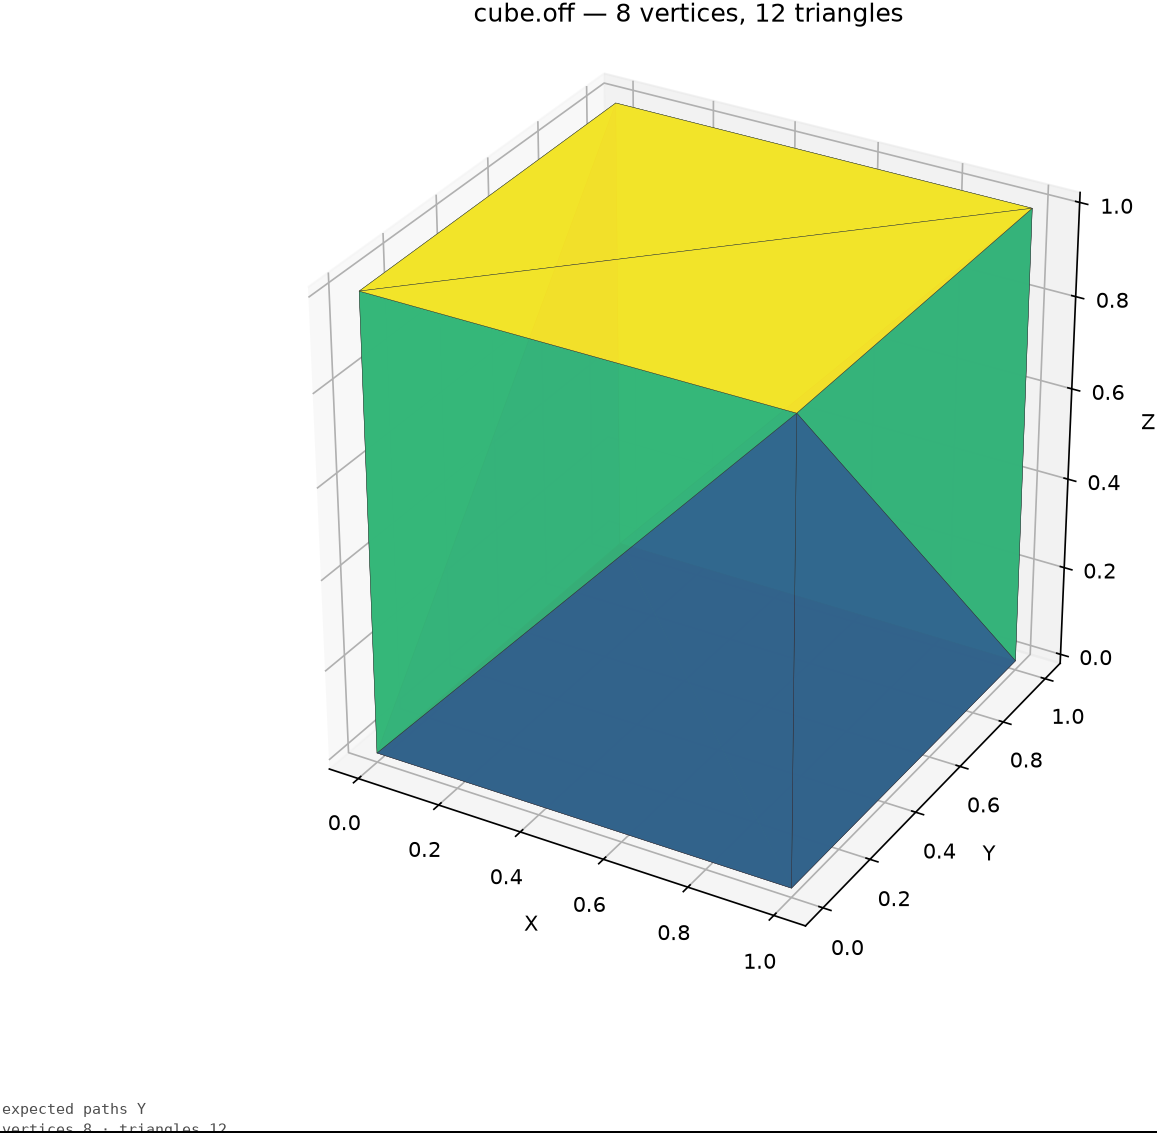
\includegraphics[width=\linewidth]{Figures/crop/repo_cube.png}
    \caption{\texttt{cube} ($V=8$, $F=12$, $s=4$)}
  \end{subfigure}\hfill
  \begin{subfigure}{0.46\textwidth}
    \centering
    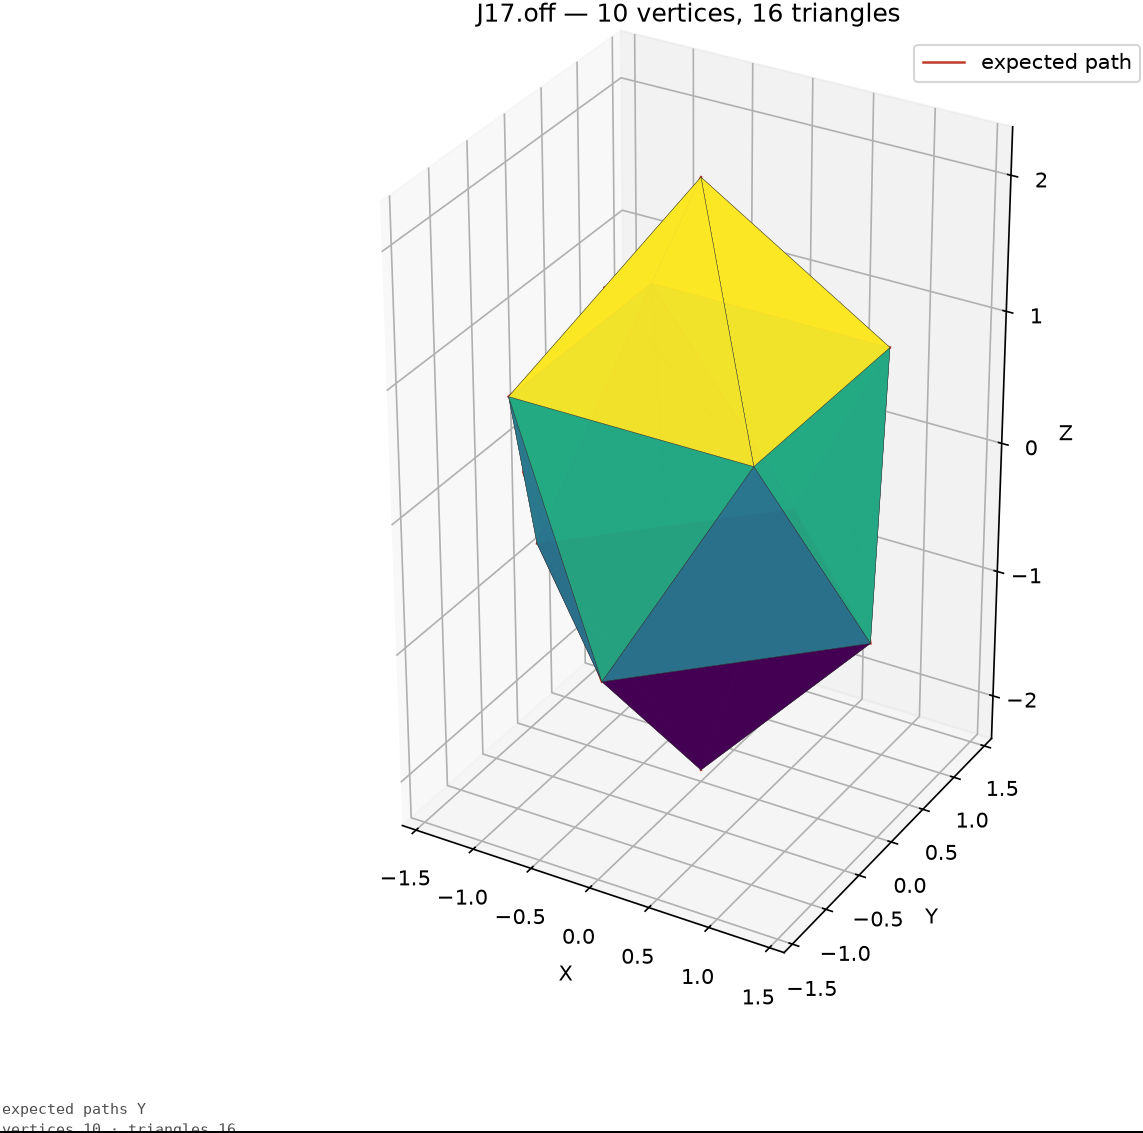
\includegraphics[width=\linewidth]{Figures/crop/repo_J17.png}
    \caption{\texttt{J17} ($V=10$, $F=16$, $s=1$)}
  \end{subfigure}\par\vspace{2pt}
  \begin{subfigure}{0.46\textwidth}
    \centering
    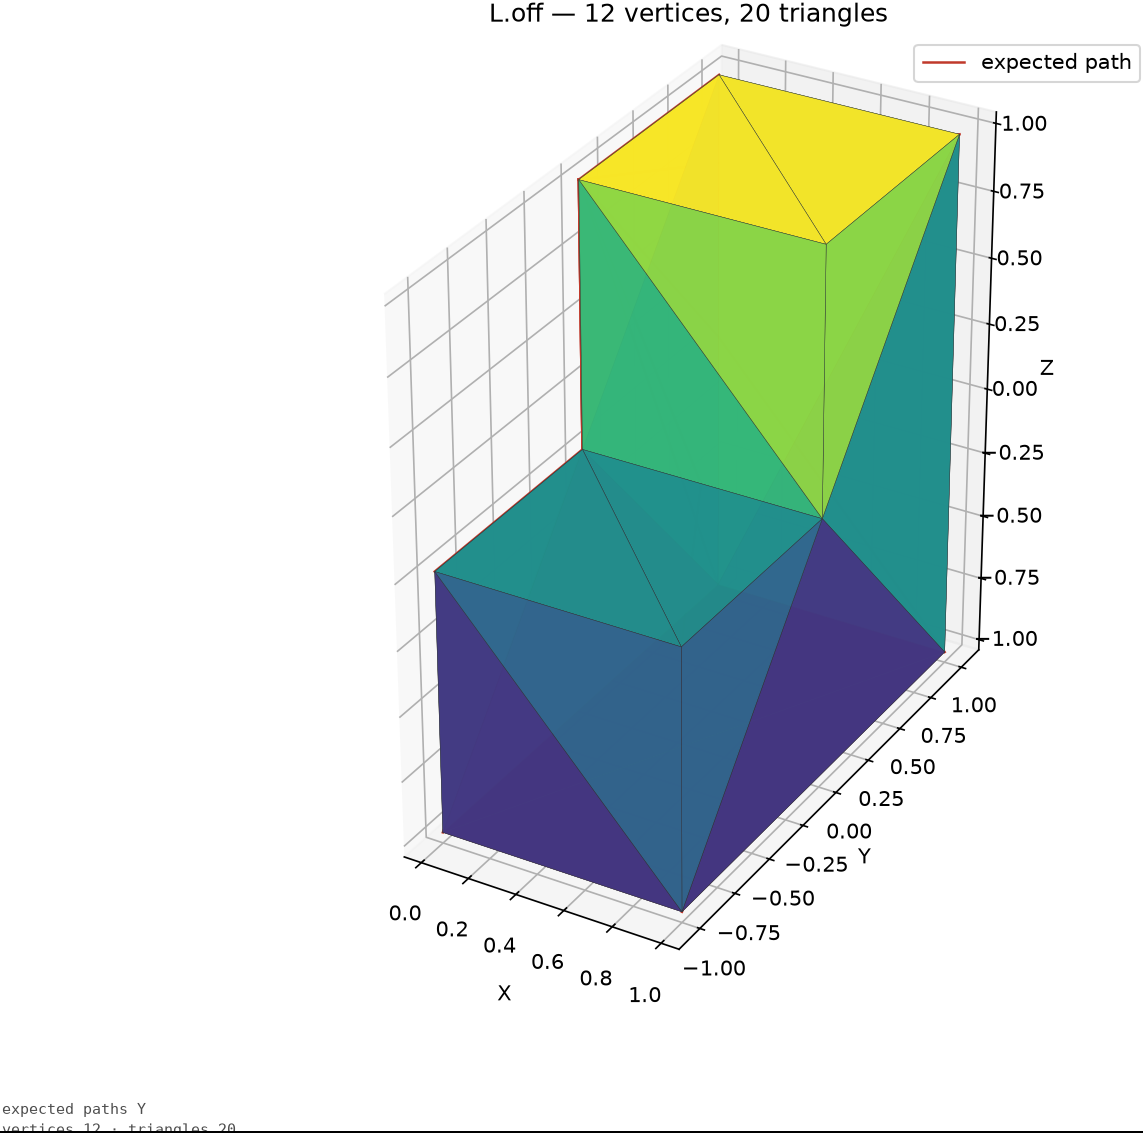
\includegraphics[width=\linewidth]{Figures/crop/repo_L.png}
    \caption{\texttt{L} ($V=12$, $F=20$, $s=1$)}
  \end{subfigure}
  \caption{Trực quan hóa ba mô hình bề mặt kín còn lại trong bộ dữ liệu, kết xuất
    từ công cụ trực quan hóa.}
  \label{fig:closed-meshes-2}
\end{figure*}

Hình~\ref{fig:closed-meshes-2} cho thấy \texttt{cube} là khối lồi đơn giản,
\texttt{J17} và \texttt{L} có các mặt phẳng nghiêng nối với nhau; cả ba đều có
đường tham chiếu đi qua mặt, không chỉ qua cạnh. Đây là các ca thuận lợi để kiểm
tra độ dài trước khi chuyển sang bề mặt phức tạp hơn.

Hình~\ref{fig:view-layers} minh họa hai lớp thông tin mà quy trình đối chiếu dùng
cho mesh \texttt{J17}: panel trái là đường tham chiếu phủ lên mesh; panel phải là
tập route do công cụ vẽ tuyến sinh, tức kết quả của Funnel Tree cho mọi đỉnh
đích. Hai panel dùng cùng dữ liệu đầu vào nhưng khác nguồn đường, nhờ đó có
thể so trực tiếp bằng mắt trước khi so độ dài ở Mục~\ref{sec:results}.

\begin{figure*}[!t]
  \centering
  \begin{subfigure}{0.46\textwidth}
    \centering
    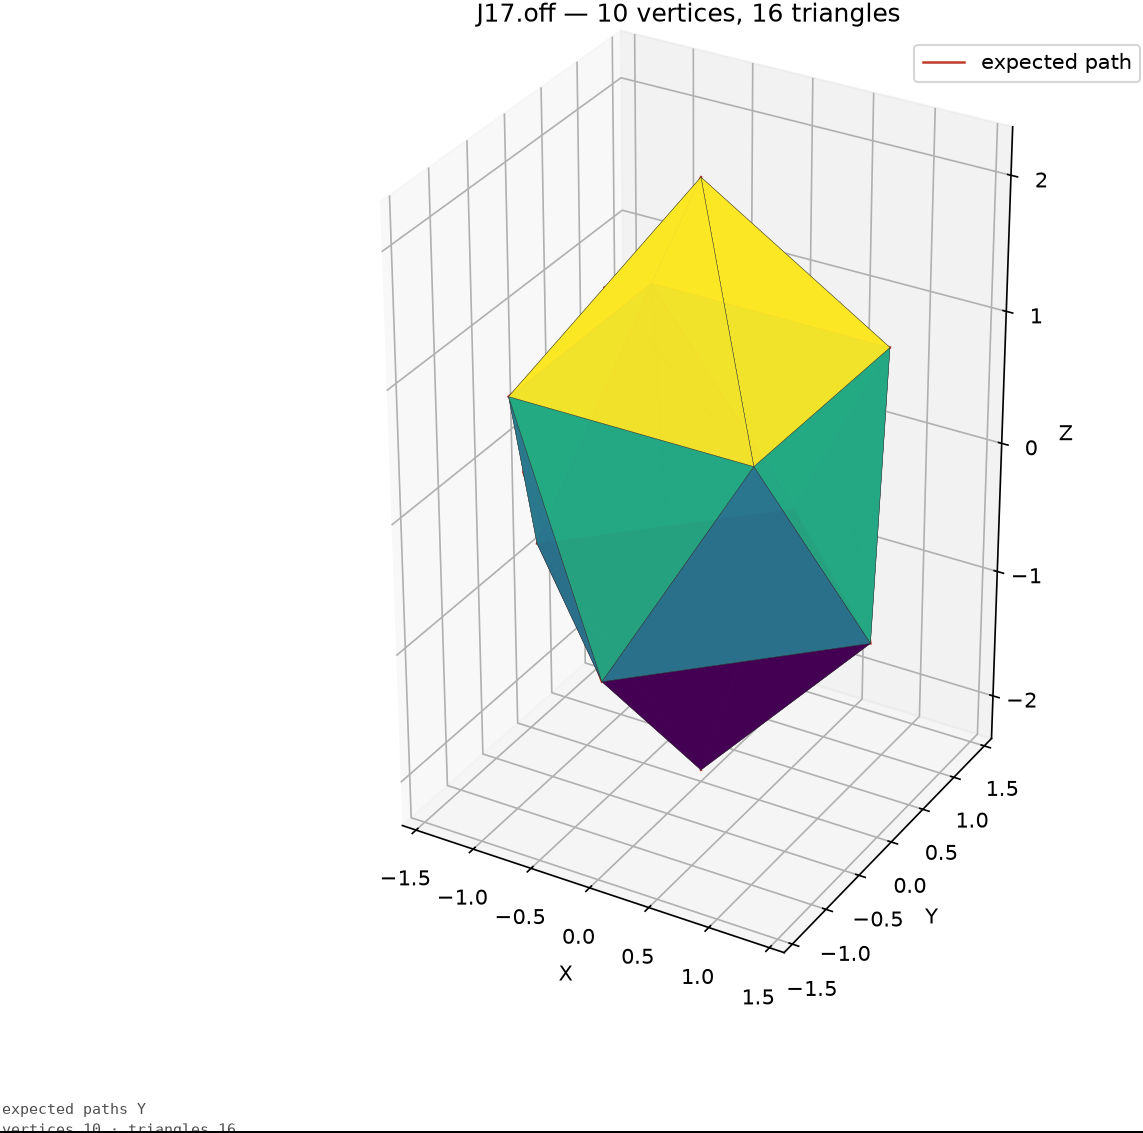
\includegraphics[width=\linewidth]{Figures/crop/repo_J17.png}
    \caption{Đường tham chiếu độc lập.}
  \end{subfigure}\hfill
  \begin{subfigure}{0.46\textwidth}
    \centering
    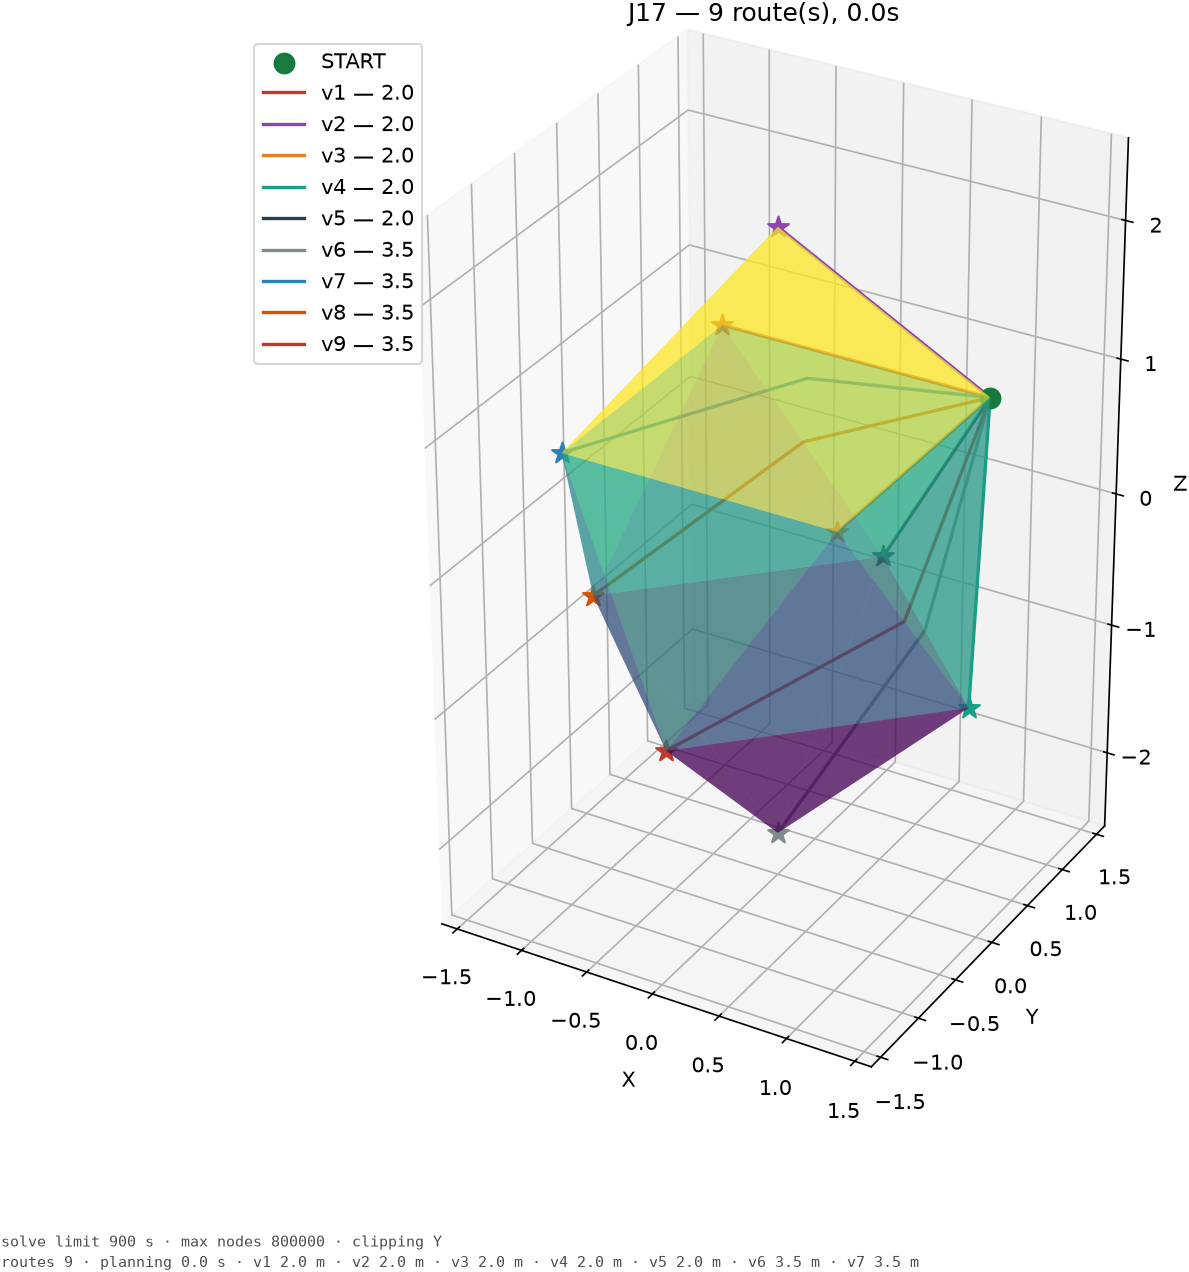
\includegraphics[width=\linewidth]{Figures/crop/repo_J17_routes.png}
    \caption{Route do Funnel Tree trả về.}
  \end{subfigure}
  \caption{Hai lớp hiển thị trên mesh \texttt{J17}: dữ liệu tham chiếu (trái) và
    kết quả Funnel Tree cho mọi đỉnh đích (phải). Cả hai ảnh đều có chân ghi
    tham số và SHA.}
  \label{fig:view-layers}
\end{figure*}

Hình~\ref{fig:open-meshes} cho thấy \texttt{dome} là một mảnh vỏ cầu khuyết
đáy còn \texttt{terrain} là mặt địa hình có thung lũng; cả hai đều có chu vi biên
hở. Các đường tham chiếu dừng ở biên thay vì đi xuyên qua, đúng ràng buộc mà thuật
toán phải xử lý.

Đối với bài toán mở rộng bề mặt mở, Hình~\ref{fig:open-meshes} trực quan hóa hai
mô hình bề mặt mở: vỏ cầu khuyết đáy \texttt{dome} và mô hình địa hình đồi núi
\texttt{terrain}. Trên các hình ảnh này, đường biên hở bao quanh mô hình thể hiện
rõ giới hạn không gian mà các tia tìm kiếm funnel không được phép vượt qua.

\begin{figure*}[!t]
  \centering
  \begin{subfigure}{0.45\textwidth}
    \centering
    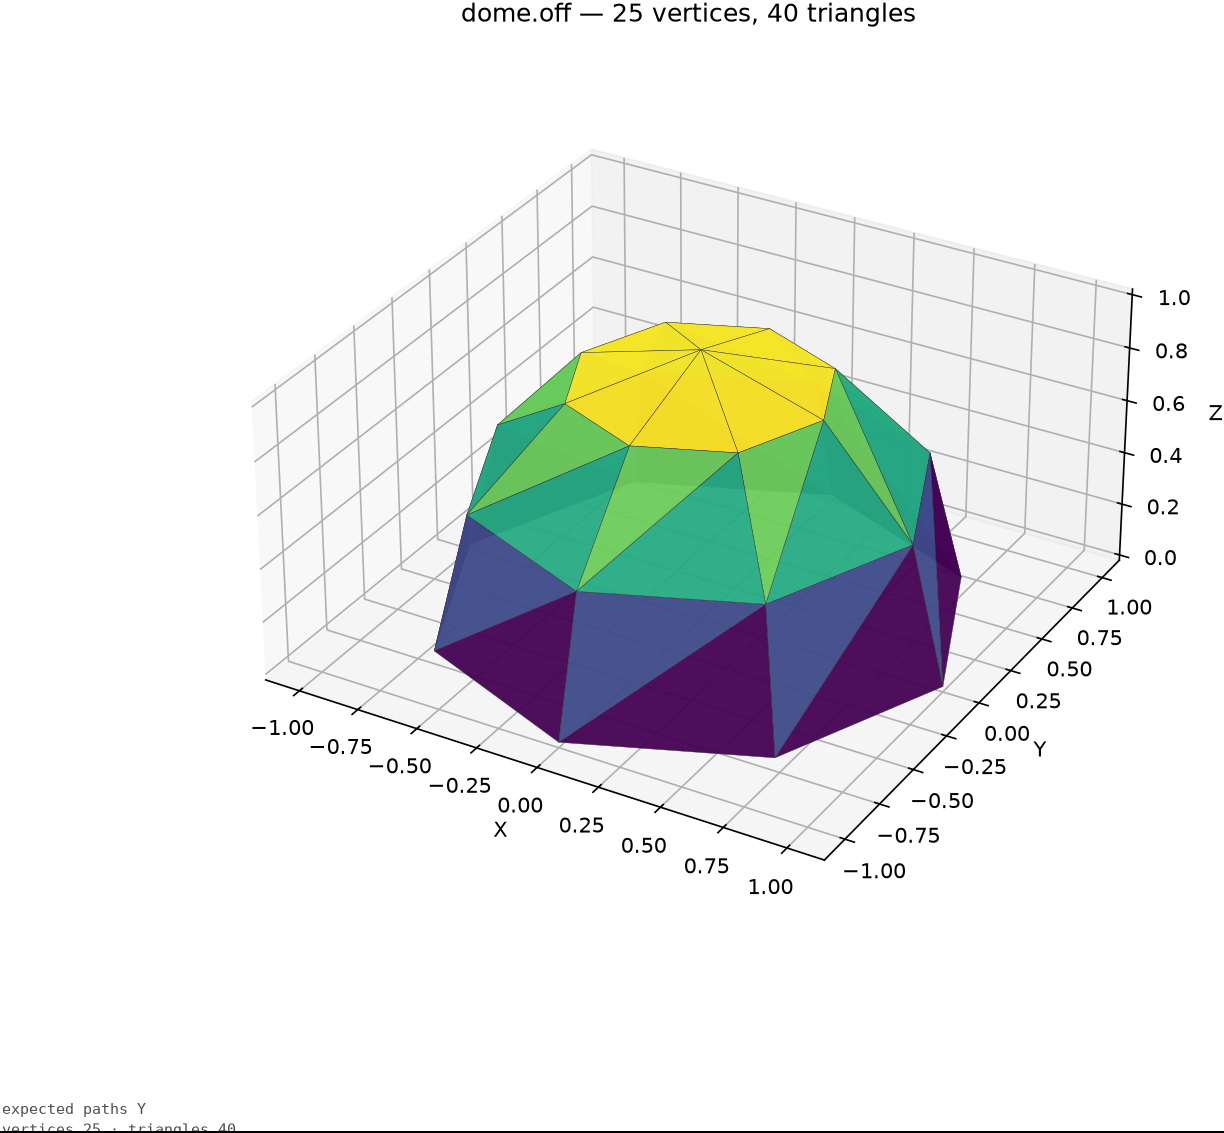
\includegraphics[width=\linewidth]{Figures/crop/repo_dome.png}
    \caption{\texttt{dome} ($V=25$, $F=40$, 8 cạnh biên)}
  \end{subfigure}\hfill
  \begin{subfigure}{0.45\textwidth}
    \centering
    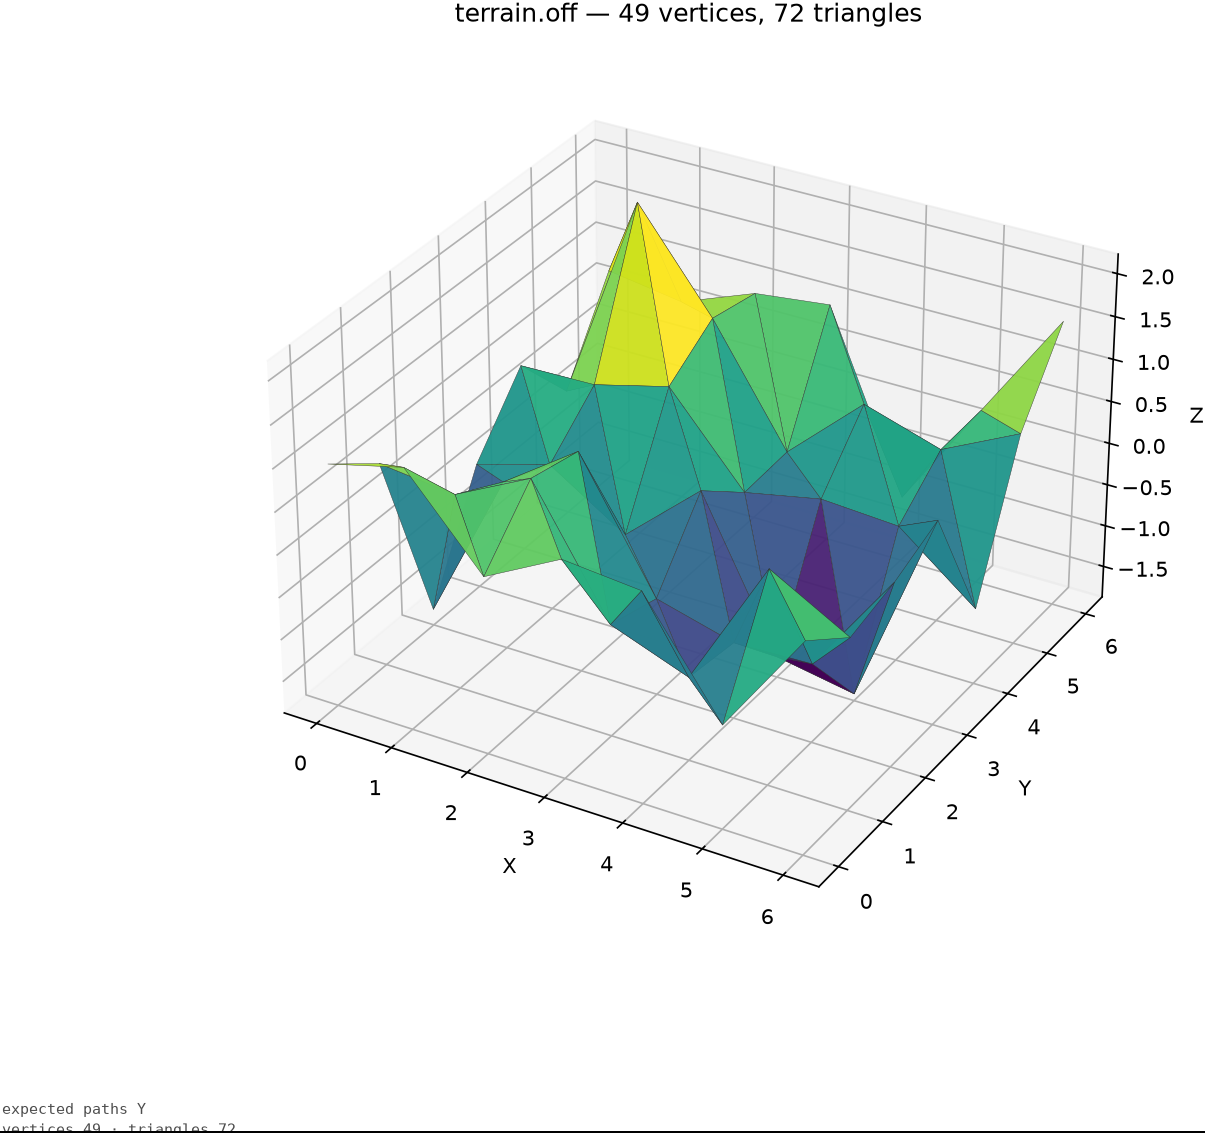
\includegraphics[width=\linewidth]{Figures/crop/repo_terrain.png}
    \caption{\texttt{terrain} ($V=49$, $F=72$, 24 cạnh biên)}
  \end{subfigure}
  \caption{Trực quan hóa hai mô hình bề mặt mở có cạnh biên, kết xuất từ
    công cụ trực quan hóa.}
  \label{fig:open-meshes}
\end{figure*}

Cuối cùng, Hình~\ref{fig:demo-mesh} biểu diễn mô hình \texttt{demo\_mesh} --- mesh
có số đỉnh và số mặt lớn nhất trong nhóm bề mặt kín, sở hữu cấu trúc tô pô dạng
xuyến ($\chi=0$) với lỗ rỗng ở trung tâm và thang đo tọa độ lớn hơn 100 lần.

\begin{figure}[!t]
  \centering
  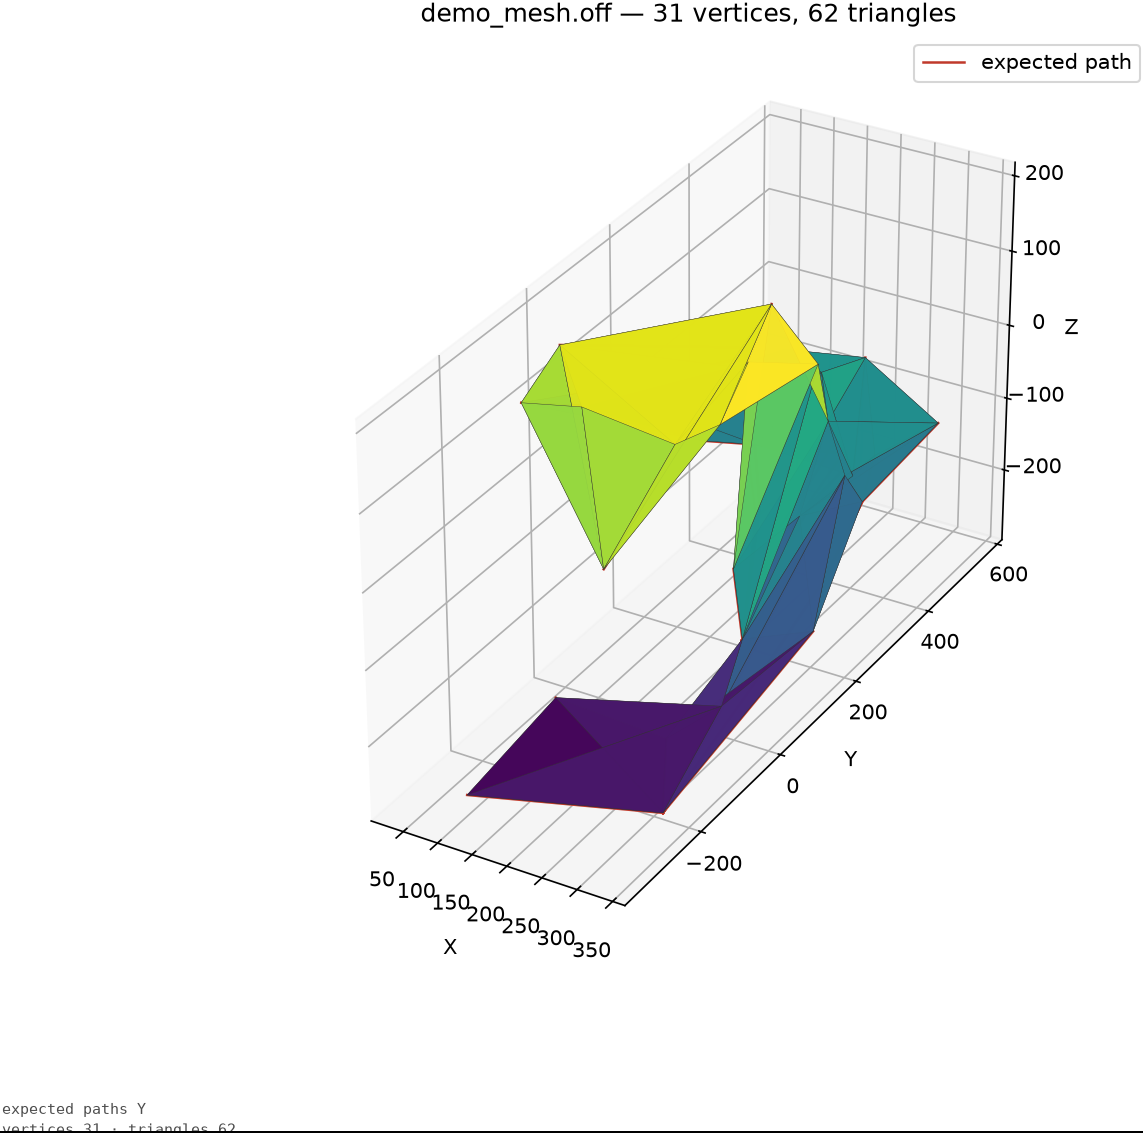
\includegraphics[width=0.95\linewidth]{Figures/crop/repo_demo_mesh.png}
  \caption{Mô hình \texttt{demo\_mesh} ($V=31$, $F=62$, $\chi=0$) dạng xuyến,
    kết xuất bởi công cụ trực quan hóa; đường tham chiếu được phủ lên mesh.}
  \label{fig:demo-mesh}
\end{figure}

Hình~\ref{fig:demo-mesh} cho thấy \texttt{demo\_mesh} có lỗ xuyên tâm và thang
tọa độ lớn hơn các mesh khác khoảng 100 lần; các đường tham chiếu vòng qua lỗ và
giữ được hình dạng xuyến. Đây là ca kiểm tra tính đúng trên bề mặt có lỗ và là lý
do mọi so sánh sai số phải dùng đại lượng tương đối.

\subsection{Insights từ EDA}

Từ các kết quả EDA và trực quan hóa dữ liệu ở trên, nghiên cứu rút ra năm insight
quan trọng, định hình trực tiếp phương pháp đánh giá thực nghiệm:
\begin{enumerate}
  \item \textbf{Dữ liệu kiểm chứng bề mặt mở đã sẵn sàng:} với sự hiện diện của
    \texttt{dome.off} (8 cạnh biên) và \texttt{terrain.off} (24 cạnh biên), kho
    mã nguồn \cite{kien2026repo} đã cung cấp đầy đủ dữ liệu để kiểm chứng thuật
    toán trên bề mặt mở (mục tiêu~3). Việc trực quan hóa ở
    Hình~\ref{fig:open-meshes} xác nhận rõ các đường biên không gian cần được xử
    lý cắt tỉa biên trong thuật toán.
  \item \textbf{Độ phong phú về dạng hình học nhưng quy mô còn nhỏ so với bài
    báo:} dữ liệu kiểm thử đã bao quát từ đa diện lồi, không lồi, dạng xuyến đến
    bề mặt mở, nhưng kích thước tối đa mới đạt $V=49$ đỉnh (so với 100--800 đỉnh ở
    \cite{an2024funnel}). Do đó, các thí nghiệm ở Mục~\ref{sec:results} đóng vai
    trò kiểm chứng tính đúng đắn và độ ổn định thuật toán, chưa phải là phép đo
    hiệu năng trên dữ liệu lớn.
  \item \textbf{Khác biệt thang đo khoảng 100 lần giữa \texttt{demo\_mesh} và các
    mesh khác:} mọi so sánh sai số ở Mục~\ref{sec:results} bắt buộc phải dùng sai
    số tương đối, không dùng sai số tuyệt đối khi đánh giá gộp các mô hình.
  \item \textbf{Độ tin cậy của output tham chiếu:} 5/9 mesh có file tham chiếu
    tham chiếu; bước đối chiếu so 76 đỉnh với
    ngưỡng tương đối $10^{-4}$ và hiện báo 0 failure. Bốn mesh còn lại không có
    tham chiếu độc lập, nên chỉ dùng để kiểm tra khả năng chạy trên bề mặt lồi,
    bề mặt mở và bề mặt có lỗ.
  \item \textbf{Mô hình thành phố \texttt{city.glb} là tiền đề cho bài toán đô thị
    thực tế:} file \texttt{city.glb} (khoảng 20,5 MB) nằm trong
    dữ liệu gốc. File này được đưa vào tính toán ở phần mô phỏng
    (Mục~\ref{sec:gazebo}), nơi mô hình thành phố được chuyển thành bề mặt dẫn
    đường tam giác hóa để lập tuyến cho UAV.
\end{enumerate}
